%%%
%
% $Autor: Wings $
% $Datum: 2021-05-14 $
% $Pfad: GitLab/MLEdgeComputer $
% $Dateiname: 
% $Version: 4620 $
%
% !TeX spellcheck = de_DE/GB
% !TeX program = pdflatex
% !BIB program = biber/bibtex
% !TeX encoding = utf8
%
%%%


\chapter{Powerbank}

\Mynote{Text fehlt}


Die Spannungsversorgung erfolgt über die Powerbank. Sie verfügt über einen Taster, mit dem sie ein- und ausgeschaltet werden kann. Zum Einschalten muss der Taster für eine Sekunden gedrückt werden. Bei kurzer Betätigung wird dem Nutzer der Ladezustand angezeigt. Zum Ausschalten muss der Taster drei Sekunden lang gedrückt werden. 

\begin{figure}[H]
    \centering
    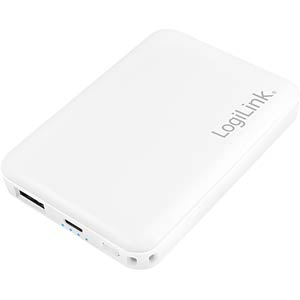
\includegraphics[width=0.8\textwidth]{Nano33BLESense/TinyMLKit/powerbank.jpg}
    \caption{Die verwendete Powerbank}
\end{figure}

\Mynote{Quelle fehlt}



